\chapter{Theory}
\label{chap:theory}

The \acf{SM} of particle physics provides an extremely successful description of all known particles and interactions. Developed in the 1960s and 70s, the \ac{SM} has survived decades of experimental tests, predicting particles before their discovery and withstanding high precision tests. However, there are several known shortcomings of the \ac{SM} that lead physicists to believe that nature must deviate from the \ac{SM} at higher energies than currently experimentally accessible. 

One attractive extension to the \ac{SM} is \acf{SUSY}, which adds an additional symmetry to the \ac{SM} between fermions and bosons, creating an additional spectrum of particles that provides solutions to the open questions in the \ac{SM}. The particular \ac{SUSY} model probed by this thesis is \acf{GMSB} \ac{SUSY}. This chapter gives an overview of the \ac{SM} and the motivation and formulation of \ac{SUSY}, it then describes \ac{GMSB} models and their current experimental context. 


\section{The Standard Model}

The \acf{SM} provides a framework for all known particles and interactions through Quantum Field Theory (QFT). Each particle is represented as a field and the dynamics as a Lagrangian ($\mathcal{L}$). All known matter particles and force carriers are described through its formulation, as is the Higgs boson. The particles of the Standard Model are divided into fermions, made up of leptons and quarks with spin-$\frac{1}{2}$, and bosons with integer spin. Matter is made of fermions and forces are mediated through spin-1 bosons, the spin-0 Higgs boson gives mass to the fermions and other bosons. The particle content of the \ac{SM} is shown in \autoref{fig:sm}. 
 
\begin{figure}[htbp]
\centering
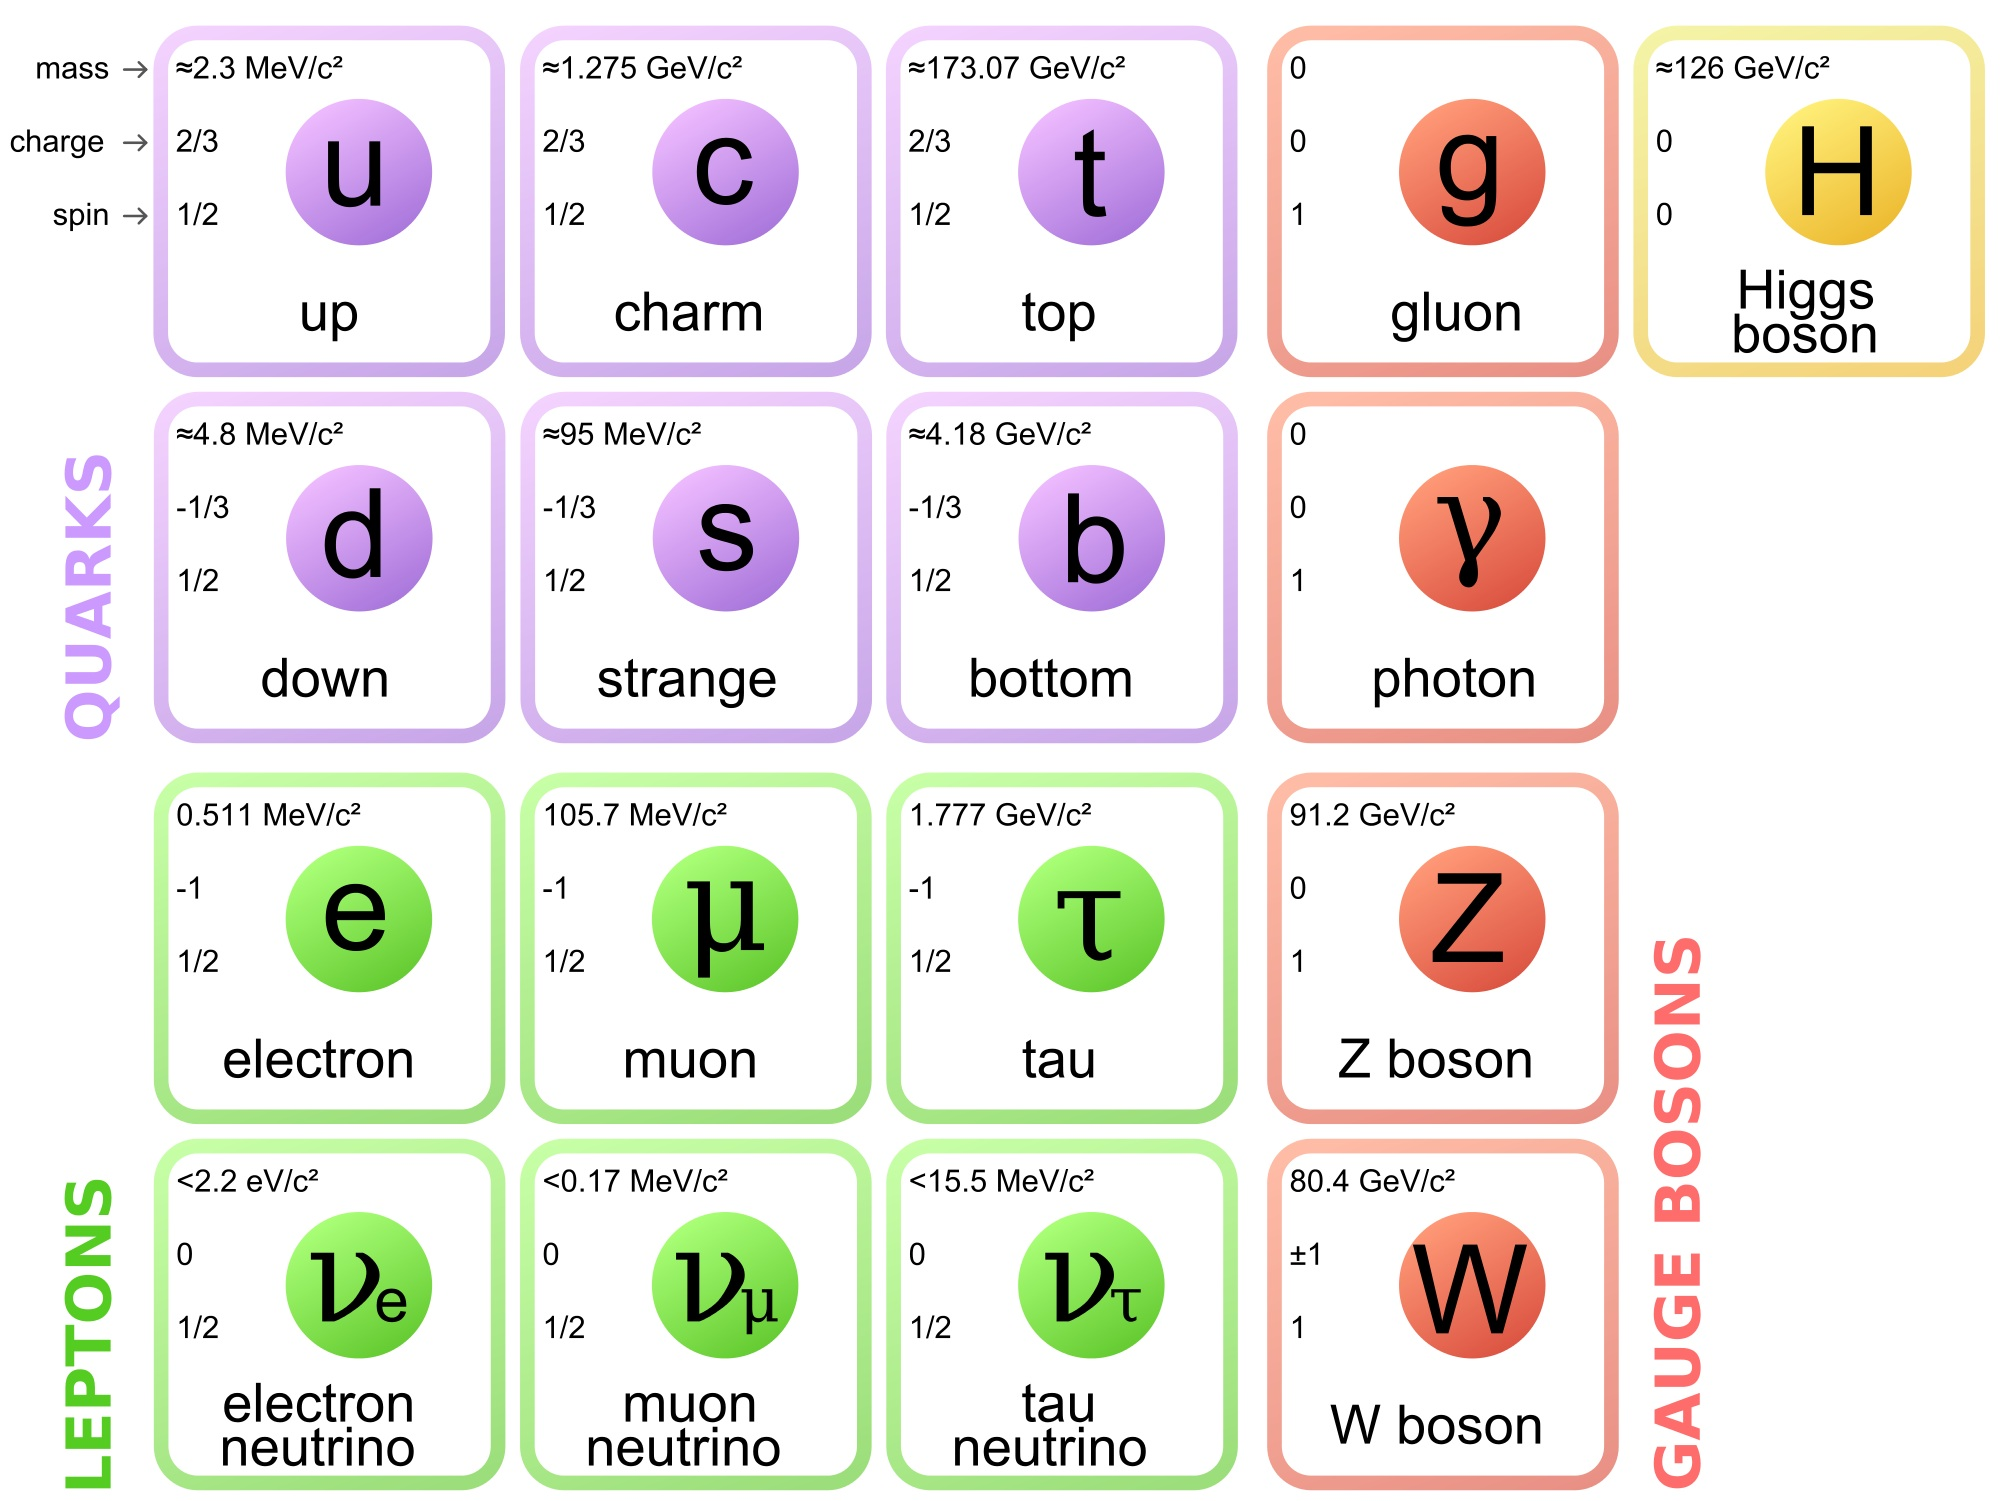
\includegraphics[width=.8\textwidth]{figures/theory/standard-model.jpg}
\caption{The particles of the Standard Model.}
\label{fig:sm}
\end{figure}



\subsection{Leptons}
There are three generations of leptons ($\ell$), labeled by flavor, which interact via the electromagnetic and weak forces: electrons ($e$), muons ($\mu$), and taus ($\tau$), ordered by mass. Each lepton has negative electromagnetic charge and has an anti-particle with positive charge. 

There are also three generations of leptons ($\nu$) which interact only via the weak force: electron neutrino ($\nu_{e}$), muon neutrino ($\nu_{\mu}$), and tau neutrinos ($\nu_{\tau}$), with unknown mass ordering. Neutrinos have no electromagnetic charge and tiny masses and thus are extremely hard to detect and not studied at the \ac{LHC}. 

Electrons and neutrinos are stable, while muons and taus are not. Muons decay to an electron and neutrino with a lifetime of 2.2 $\mu$s, and taus decay 17\% of the time each to an electron or muon and neutrinos, and the remaining 66\% of the time into hadrons and neutrinos. In any \ac{SM} process, the number of leptons ($L$) of each flavor is conserved. 


\subsection{Quarks}
There are three generations of quarks that interact via the electromagnetic, weak, and strong forces. Quarks are further divided into up-type with charge $+\frac{2}{3}q_{e}$ and down-type (with charge $-\frac{1}{3}q_{e}$). The up-type quarks are up ($u$), strange ($s$), and bottom ($b$), the down-type quarks are down ($d$), charm ($c$) and top ($t$). Since they also interact via the strong force, each quark also has a color charge, either red, blue, or green (or the opposite (anticolor)). Individual quarks are not seen in nature and all stable particles are color neutral with whole number charges, either a mix of all three colors or color and anticolor. In nature, quarks are found in color-neutral composite particles called \emph{hadrons}. Color-anticolor pairs are called \emph{mesons} and states with all three colors are called \emph{baryons}. The lightest hadron, the proton ($uud$), is stable, but all others are not with a wide range of lifetimes. For example, free neutrons ($udd$) have a lifetime of about 15 minutes; pions ($u\bar{u}$) have a lifetime of 26 ns and can travel a substantial distance at the speed of light before decaying; b-mesons a lifetime of 1.5 ps and travel shorter distances if produced in collisions; all other hadrons have shorter lifetimes. 

Similar to leptons, the baryon number ($B$) is preserved in the \ac{SM}. Baryons have $B = 1$, anti-baryons $B=-1$, and mesons $B=0$.

While quarks can result from \ac{LHC} interactions, color confinement means that bare quarks are not observed by the detectors.

\subsection{Forces}

The electromagnetic, strong, and weak interactions result from the exchange of bosons between the fermions that make up matter. Force mediators interact with fermions that are charged under the corresponding force's quantum numbers. Gravity is not described by the Standard Model because its relative interaction strength is so small.

The symmetries of the Standard Model dictate its possible interactions. The Standard Model must invariant under choice of gauge. To accomplish this, gauge fields are added to the Lagrangian to cancel out the gauge dependence of the free Lagrangian. The gauge fields must be massless or a Higgs field must be introduced in order to maintain the gauge invariance. The Higgs field gives masses to the weak gauge bosons.

The \ac{SM} Lagrangian in invariant symmetries, or local gauge transformations. The symmetry group of the Standard Model is 
\begin{equation}
SU_{C}(3) \times SU_{L}(2) \times U_{Y}(1) 
\end{equation}
where $C$ stands for the color charge of the strong force, $L$ stands for left because the weak force is left-handed, and Y stands for \emph{hypercharge}, the quantum number of the electroweak force. ``Left-handed'' describes a particle whose spin is oriented opposite its direction of motion. 


\begin{table}[htb]
\begin{center}
\begin{tabular}{cc}
 force & relative coupling strength \\
 \hline
  gravity   &  $10^{-39}$    \\
  weak      &  $10^{-6}$     \\
  electromagnetic  &  $\frac{1}{137} $   \\
  strong  &  1     \\
\hline
\end{tabular}
\caption{The relative strength of the fundamental forces.}
\end{center}
\end{table}


\subsubsection{Electroweak Force}
The electromagnetic and weak forces are low-energy manifestations of the unified electroweak force. The $SU_{L}(2) \times U_{Y}(1)$ symmetry group of the \ac{SM} generates the electoweak force. If the gauge bosons were massless, $SU_{L}(2)$ alone would describe their interactions. The quantum number of the electroweak force is hypercharge, defined as
\begin{equation}
Y=2(Q-T_{3})
\end{equation}
where $Q$ is the electromagnetic charge and $T_3$ is the third component of the electroweak isospin, the quantum number of the weak interaction.

The gauge bosons that result from the $SU_{L}(2) \times U_{Y}(1)$ symmetry include a triplet and singlet field. The symmetry is broken, these states mix and the electroweak force carriers are produced: $W^{\pm}$ from two of the triplet states, and the $Z$ and photon result from the mixing of the last triplet state with the singlet.

\paragraph{Electromagnetic Force}

Fermions with electric charge interact via the electromagnetic force mediated by the photon ($\gamma$). The photon is massless. Being chargeless and spin-1, photons can \emph{pair-produce} a fermion and anti-fermion if the photon's energy is more than twice the rest mass energy of the fermion. Specifically, photons from \ac{LHC} collisions can pair produce electrons and are called \emph{conversions} or \emph{converted photons}.

\paragraph{Weak Force}
All fermions are charged under the weak force, mediated by the $W^{\pm}$ and $Z$ bosons. The $W$ bosons interact with left-handed particles and right-handed anti-particles, while the $Z$ boson interacts with both left- and right-handed particles. $W$ bosons are charged so they also interact with photons. The $W$ boson has mass of 80.4 GeV and the $Z$ boson of 90.2 GeV. The coupling constant of the weak force is about $10^{5}$ smaller than that of the electromagnetic force.

\subsubsection{Strong Force}
Fermions with color charge interact under the strong force, generated by the $SU_{C}(3)$ symmetry and mediated by the massless gluon. The gluon itself is color charged, so gluons interact with each other, and the strength of the color force, the strong coupling constant $\alpha_s$ increases as a function of distance.  $\alpha_s$ also evolves as a function of energy scale $\mu$ as
\begin{equation}
\alpha_s(\mu)= \frac{12\pi}{(32-2n_f)\text{ln}\frac{\mu^2}{\Lambda^2_{\text{QCD}}}}
\end{equation}
where $n_f$ is the number of quarks flavors (6) and $\Lambda_{\text{QCD}}$ is the the cutoff scale (about 0.2 GeV).



These features of $\alpha_s$ have several important consequences. The first is \emph{color-confinement}. If two quarks are pulled apart, $\alpha_s$ increases and so does the amount of energy required to continue to separate them. Eventually, it becomes energetically favorable to produce a quark-antiquark pair and form two mesons, rather than continue to separate the original quarks. The result of pulling apart the two quarks is not two separated, colored quarks, but two color-neutral hadrons.

Because of this, quarks that result from interactions in the \ac{LHC} cannot be directly observed. If one is produced it first undergoes a \emph{parton shower}, creating many new colored particles along its trajectory until the particles have enough energy to \emph{hadronize} and form color-neutral particles. This spray of color-neutral hadrons is observed in detectors, and the detector signatures are grouped into a \emph{jet}.

Conversely, at very small distances ($< 10^{-16}$ m), the strong coupling is very small, and so quarks inside of hadrons can move around freely. In this regime, \ac{QCD} can be described perturbatively. $\Lambda_{\text{QCD}}$ is the energy scale at which $\alpha_s$ is too large for perturbation theory to apply.


\subsection{Higgs Boson}

The Higgs boson is the only spin-0 particle in the Standard Model and gives the mass to the gauge bosons via electroweak symmetry breaking and to the fermions via the Yukawa coupling. The addition of the $U(1)$ symmetry group results in a massive gauge field (the electroweak triplet) and a massive scalar (the Higgs). The Higgs can also interact with itself.

Nothing in the \ac{SM} dictates the mass of the Higgs boson. The only known mass scale not yet exploited is the Planck scale, $M_P ~{} 10^{19}$ GeV. The mass of the Higgs boson has been measured experimentally at around $125$ GeV. The difference between the measured Higgs boson mass and the Planck scale is known as the \emph{heirarchy problem}, which suggests that there is an undiscovered physics scale lower than $M_P$. 


\subsection{Conserved Quantities}

In addition to the gauge symmetry that necessitates the existence of the W and Z bosons, the other symmetries of the Standard Model dictate how its particles interact. Symmetry over translations in time lead to conservation energy, translations in space to conservation of momentum, and rotations in space to conservation of angular momentum. Lorentz invariance leads to the conservation of CPT, the combination conservation of charge, parity, and time. There are other conserved quantities that do not arise from known symmetries of the \ac{SM}, including baryon number $B$ and lepton number $L$. 


\subsection{Shortcomings}
There are many reasons to believe the Standard Model does not give a full picture of fundamental physics, despite its robustness against experimental examination. Perhaps the most obvious hole is the lack of a description of gravity. General Relativity provides an extremely effective description of gravity at large scales, but no such description exists at quantum scales. Gravitational interactions become important at $M_P$, well beyond the reach of current experiments and many orders of magnitude larger than the weak scale. Additionally, dark matter and neutrino masses have been observed experimentally, but have no explanation in the Standard Model. 

There are also several aesthetic features of the Standard Model that indicate something might be missing, but are not real problems with the theory. The hierarchy problem suggests that there should be another mass scale below the Planck scale to control the Higgs boson mass. The experimentally measured mass is the sum of the bare mass that appears in the Lagrangian and any quantum corrections from interactions with other particles. Should there be no lower mass scale, those quantum corrections would need to be $10^{35}$ times larger than the Higgs mass. While this is possible, the idea of combining two very large numbers to result in exact, small number makes physicists very uncomfortable and indicates that there might be something that is not understood.

\todo{force unification}


\section{Supersymmetry}

\acf{SUSY} is a theory proposed and developed in the 1970s \cite{susy-found-1,susy-found-2,susy-found-3} that provides solutions to many of the problems with the \ac{SM}. \ac{SUSY} adds a symmetry in addition to the ones already discussed: a symmetry between fermions and bosons whereby fermions can be changed to bosons and vice versa. 

In \ac{SUSY}, each \ac{SM} particle gets a \emph{superpartner} with all of the same quantum numbers except for spin. The bosonic superpartners of fermions are \emph{sfermions} and the fermionic partners of the \ac{SM} bosons have ``-ino'' appended to their names. For example, the superpartner of a tau $\tau$ lepton is a stau $\stau$ and the superpartner of a gluon $g$ is the gluino $\tilde{g}$. A \emph{supermultiplet} refers to the pair of the \ac{SM} particle and its superpartner.

Should \ac{SUSY} exist, we already know that it must be broken. If the selectron had the same mass as the electron it would have been observed decades ago, so superpartners must be heavier than their \ac{SM} counterparts. The mechanism by which \ac{SUSY} can be broken depends on the specific \ac{SUSY} model.

\subsection{Minimal Supersymmetric Standard Model}

\todo{particle content}
\todo{define LSP, NSLP}
\todo{R-parity}
\todo{susy breaking}

\subsection{Simplified Models}

\subsection{GMSB}

There are various mechanisms by which \ac{SUSY} can be broken. In \acf{GMSB} models, the symmetry breaking occurs via ordinary gauge interactions by heavy messengers carrying $SU(3) \times SU(2) \times U(1)$ quantum numbers \cite{gmsb-lep,Dimopoulos_1996,Ambrosanio_1997}.

Phenomenologically, \ac{GMSB} models have several notable features. 
\begin{itemize}
	\item The \ac{LSP} is always the gravitino $\tilde{G}$ because it does not get its mass through the gauge interactions. $m_{\tilde{G}}$ is related to $F/M_P$, where $\sqrt{F}$ is the \ac{SUSY} breaking scale ($\tilde{} 10^4 - 10^{11}$ GeV) and $M_P$ is the Planck scale ($\tilde{} 10^{19}$ GeV), making the mass extremely small and can be approximated as massless.

	\item The \ac{NLSP} is either the lightest neutralino $\chi$ or the slepton \slep. In the slepton case, the \ac{NLSP} is either the stau \stau or all three flavors \selec, \smu, \stau are mass degenerate co-\acp{NLSP}s. The \ac{NLSP} decay modes are $\chi \rightarrow \gamma \tilde{G}$ or $\tilde{\ell} \rightarrow \ell \tilde{G}$. This thesis presents a search for the  \slep. 

	\item Due to the small gravitational coupling, the decay is suppressed and the \ac{NLSP} becomes \emph{long lived}. 
\end{itemize}


\begin{figure}[htbp]
\centering
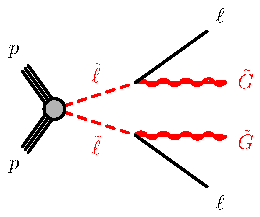
\includegraphics[width=.8\textwidth]{figures/theory/slsl-llGG-GMSB.pdf}
\caption{\ac{GMSB} \slep decay to \ac{SM} $\ell$ and $\tilde{G}$. This is the Feynman diagram targeted by the search presented in this thesis.}
\label{fig:feynman}
\end{figure}


The lifetime of a slepton \ac{NLSP} can be expressed as
\begin{equation}
   c \tau \approx 100 \um \bigg(\frac{100 \GeV}{m_{\slep}}\bigg)^5\bigg(\frac{\sqrt{F}}{100 \TeV}\bigg)^4
\end{equation}
Even at the low end of possible \ac{SUSY} breaking scales, the \slep will travel a substantial distance relative to \ac{SM} particles \cite{jesseshelton}. Particle lifetimes will be further discussed in \autoref{chap:llps}. In the intermediate breaking scale regime, the \slep can travel a small distance before decaying resulting in \ac{SM} $\ell$ are \emph{displaced} meaning they originate a macroscopic distance from the \slep production point. Most \ac{SUSY} searches at colliders assume that leptons are \emph{prompt} and point back to the \slep production point and have no sensitivity to \slep with long lifetimes. Long lived \slep production was last explored by the OPAL experiment at \ac{LEP} which excluded models with \slep masses less than 90 GeV. Experimental context for this search will be further discussed in \autoref{chap:context}.

The search presented in this thesis provides unique sensitivity to \ac{GMSB} \slep decays. The signature of the decay is a displaced \ac{SM} $\ell$, either two electrons, two muons, or an electron and a muon. The range of possible $\ell$ masses and lifetimes to which this search is sensitive is dictated by:
\begin{itemize}
	\item The \emph{cross section} of \slep production, or the probability that it will occur in a $pp$ collision. The cross section decreases with increasing \slep mass. This signature is not expected to have backgrounds from \ac{SM} processes, so only 3 events must be observed to make a discovery. This sets an upper bound on the mass sensitivity.
	\item The size of the detector and reconstruction algorithms dictate lifetime sensitivity. In this search, the trajectory of the lepton must be measured in the tracking detector and that trajectory must be substantially displaced. This requirement sets the upper and lower bounds of lifetime sensitivity.
	\item The requirement that both \ac{SM} $\tau$ decay leptonically limits the \stau sensitivity relative to \selec and \smu. 12\% of di-$\tau$ events have both $\tau$ decaying leptonically. 
	\item The thresholds for triggering an event during data collection set a lower limit on mass sensitivity. These thresholds will be further discussed in \autoref{sec:daq}. This particularly limits the \stau sensitivity for two reasons. First, electrons and muons from \stau decays have lower momentum than leptons resulting from \selec or \smu because some of the $\tau$ momentum is carried away by the neutrinos in the decay. Additionally, the \stau \ac{NLSP} is expected to be right-handed which results in lower energy $\tau$, shown in \autoref{fig:taupt}. 
\end{itemize}


\begin{figure}[htbp]
\centering
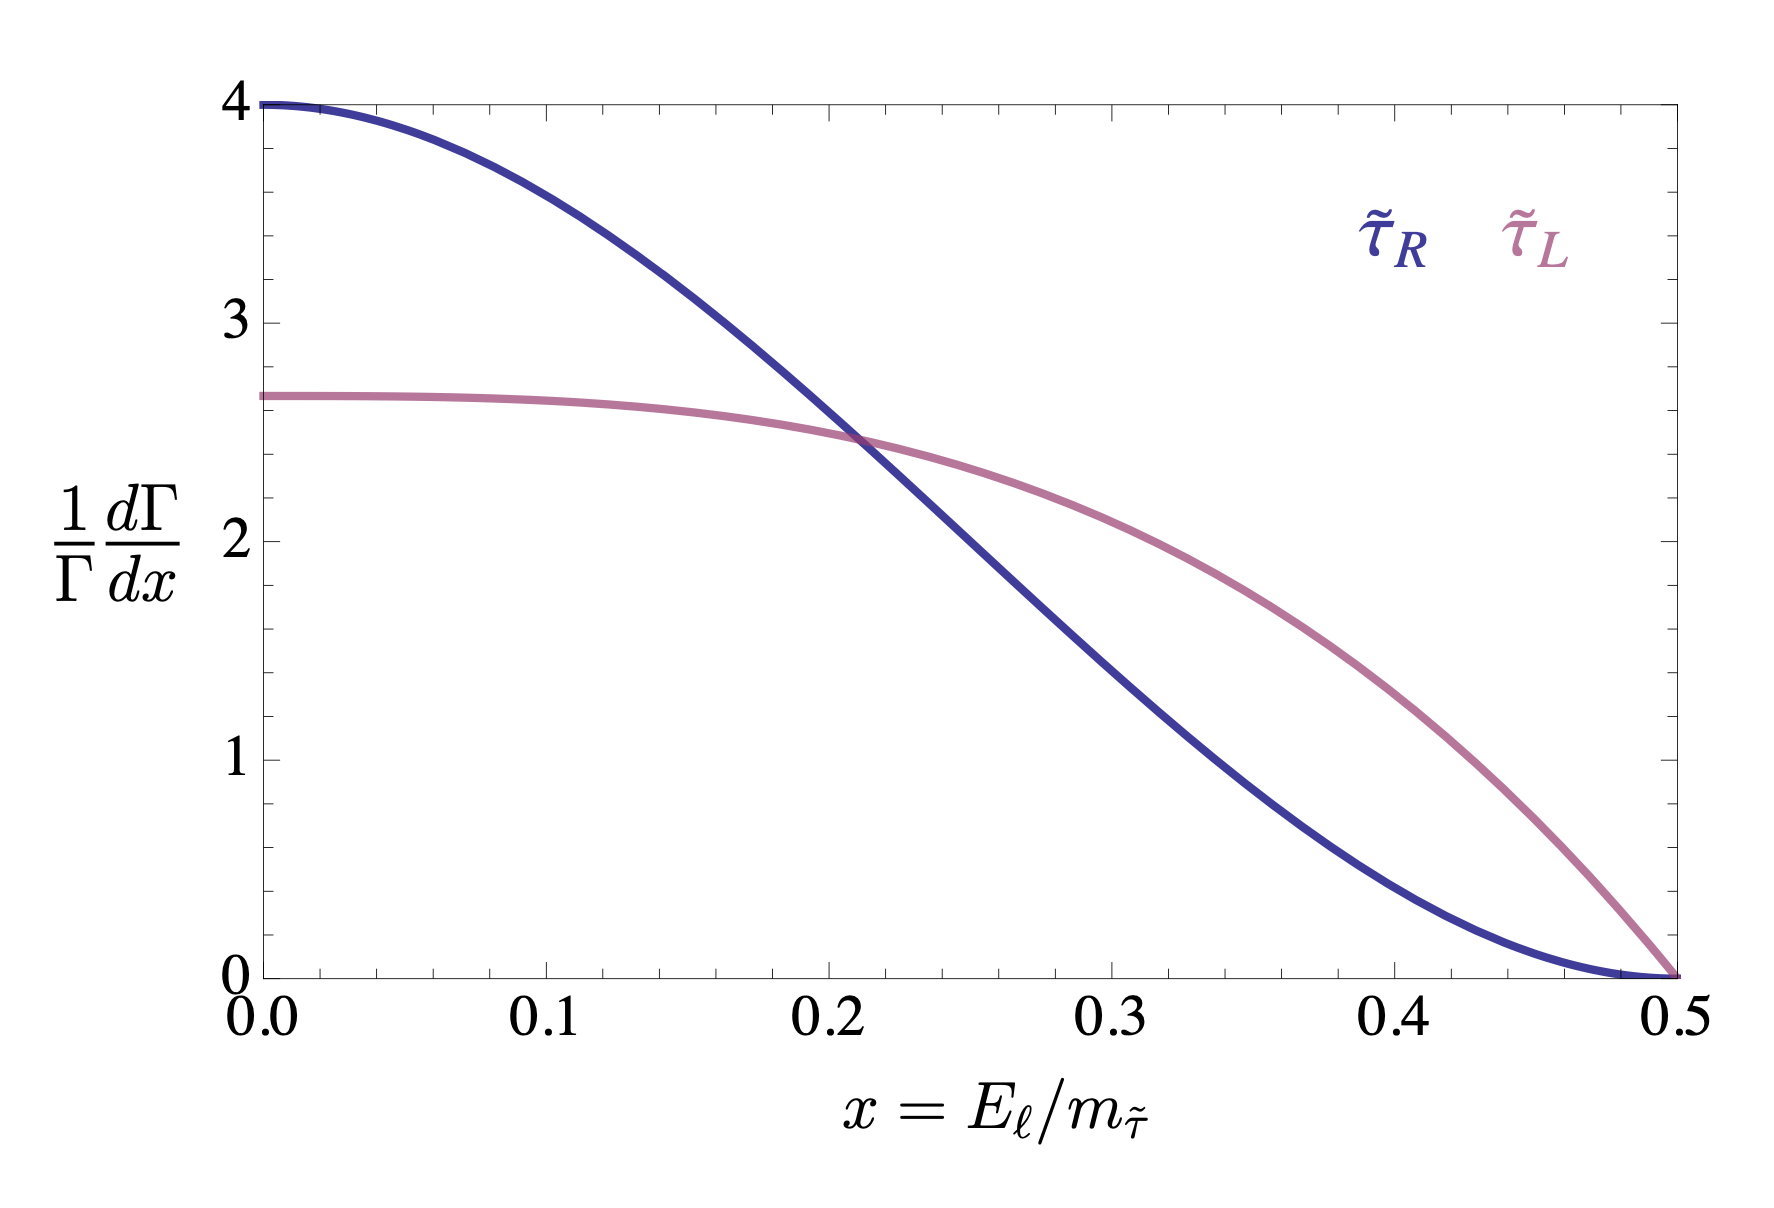
\includegraphics[width=.8\textwidth]{figures/theory/tau-pt.png}
\caption{Distribution of $\tau$ energies from left- and right-handed \stau decays. A \ac{GMSB} \stau is expected to be right-handed, resulting in lower $\tau$ energies.}
\label{fig:taupt}
\end{figure}

This search is sensitive to \selec and \smu with masses 50--800 GeV and lifetimes 0.001--10 ns, and \stau with masses 100--400 GeV and lifetimes 0.01--1 ns.



